\section{Results}
\subsection{Random Forest}
Our first task is to train Random Forest models. We use the default CART random forests from Tensorflow. In the first part, we compare two versions of the random forests:

\begin{itemize}
    \item Passing raw data to the model
    \item Preprocessing the data by encoding the Gender, Attendance and Grade columns into numbers. For example, Grade A goes to 0, A- goes to 1 and so on.
\end{itemize}


We train Random Forests with the default hyperparameter values for \texttt{num\_trees} and \texttt{max\_depth}.\\\\

\begin{tabular}{|p{4cm}||p{2 cm}||p{3cm}||p{3cm}|}
\hline
\multicolumn{4}{|c|}{\texttt{num\_trees}=300, \texttt{max\_depth}=16}\\
\hline
\textbf{Pre-processing} & \textbf{Train-Test split} (\%) &\textbf{Training OOB Accuracy (\%)} & \textbf{Testing OOB Accuracy (\%)} \\
\hline
Raw & 100 : 0& 96.39& -\\
\hline
Gender, Attendance, Grade encoded & 100 : 0  & 97.00&- \\
\hline
Raw & 70 : 30&  94.74& 86.33 \\
\hline
Gender, Attendance, Grade encoded & 70 : 30  &94.69 & 83.85 \\
\hline
\end{tabular}\newline


\subsection{Tree Visualization}

This is the first tree in the Random Forest constructed on data after the \textbf{70-30 split} and encoding of categorical attributes. It is built using the \texttt{dtreeviz} module.


\newpage
% \begin{sidewaysfigure}[ht]
%     \centering
%     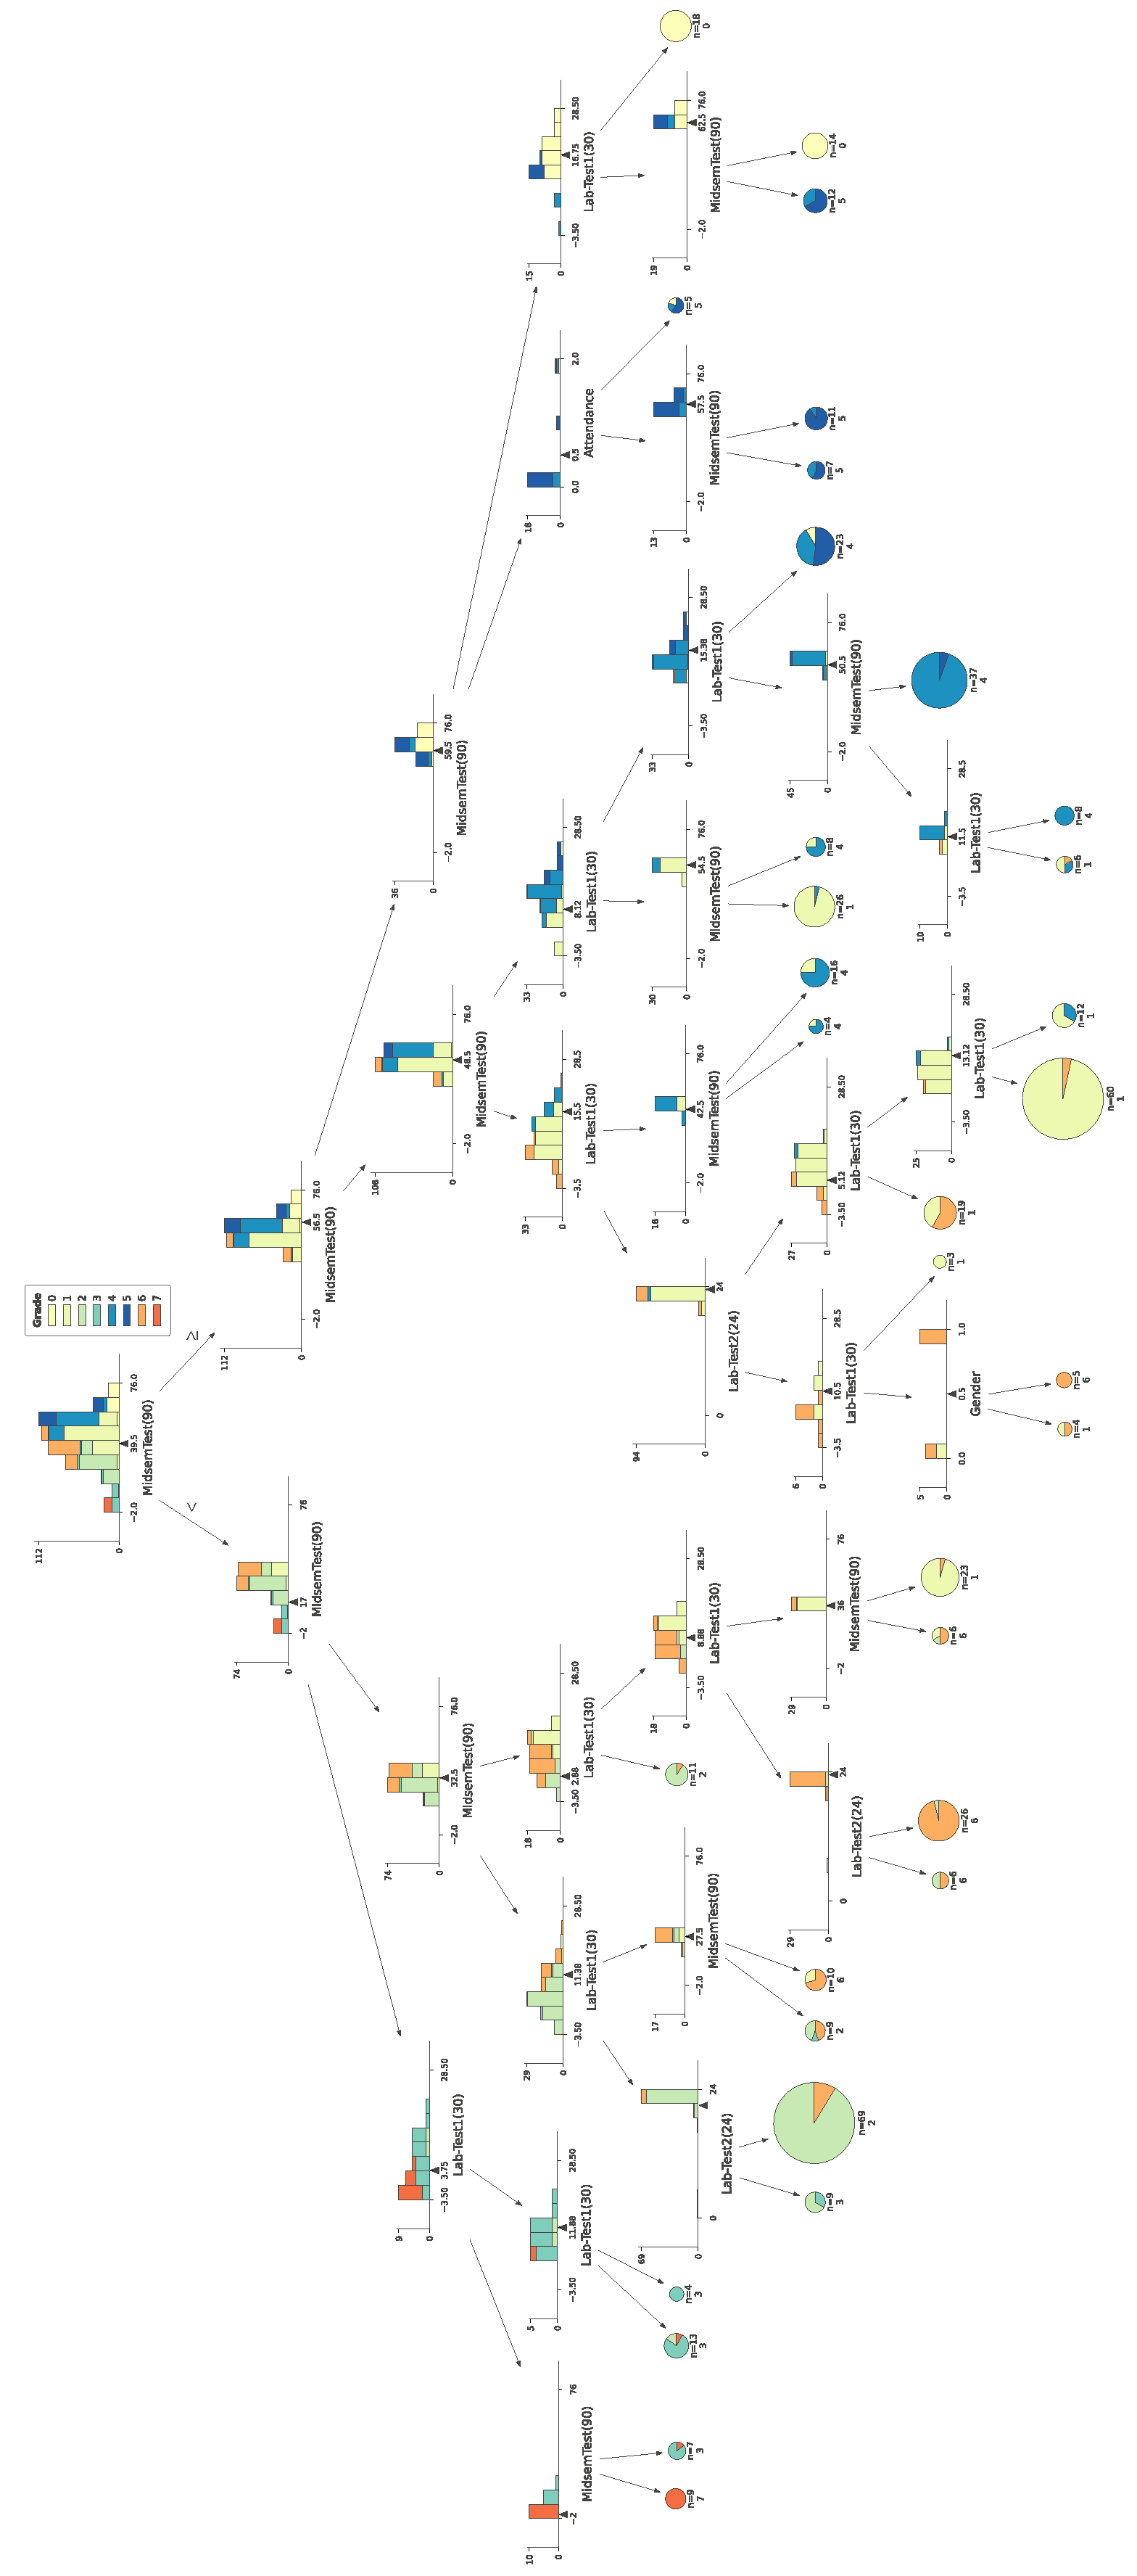
\includegraphics{images/rf_viz_cmodel.pdf}
%     \caption*{Decision Tree}
%     \label{fig:your_label}
% \end{sidewaysfigure}
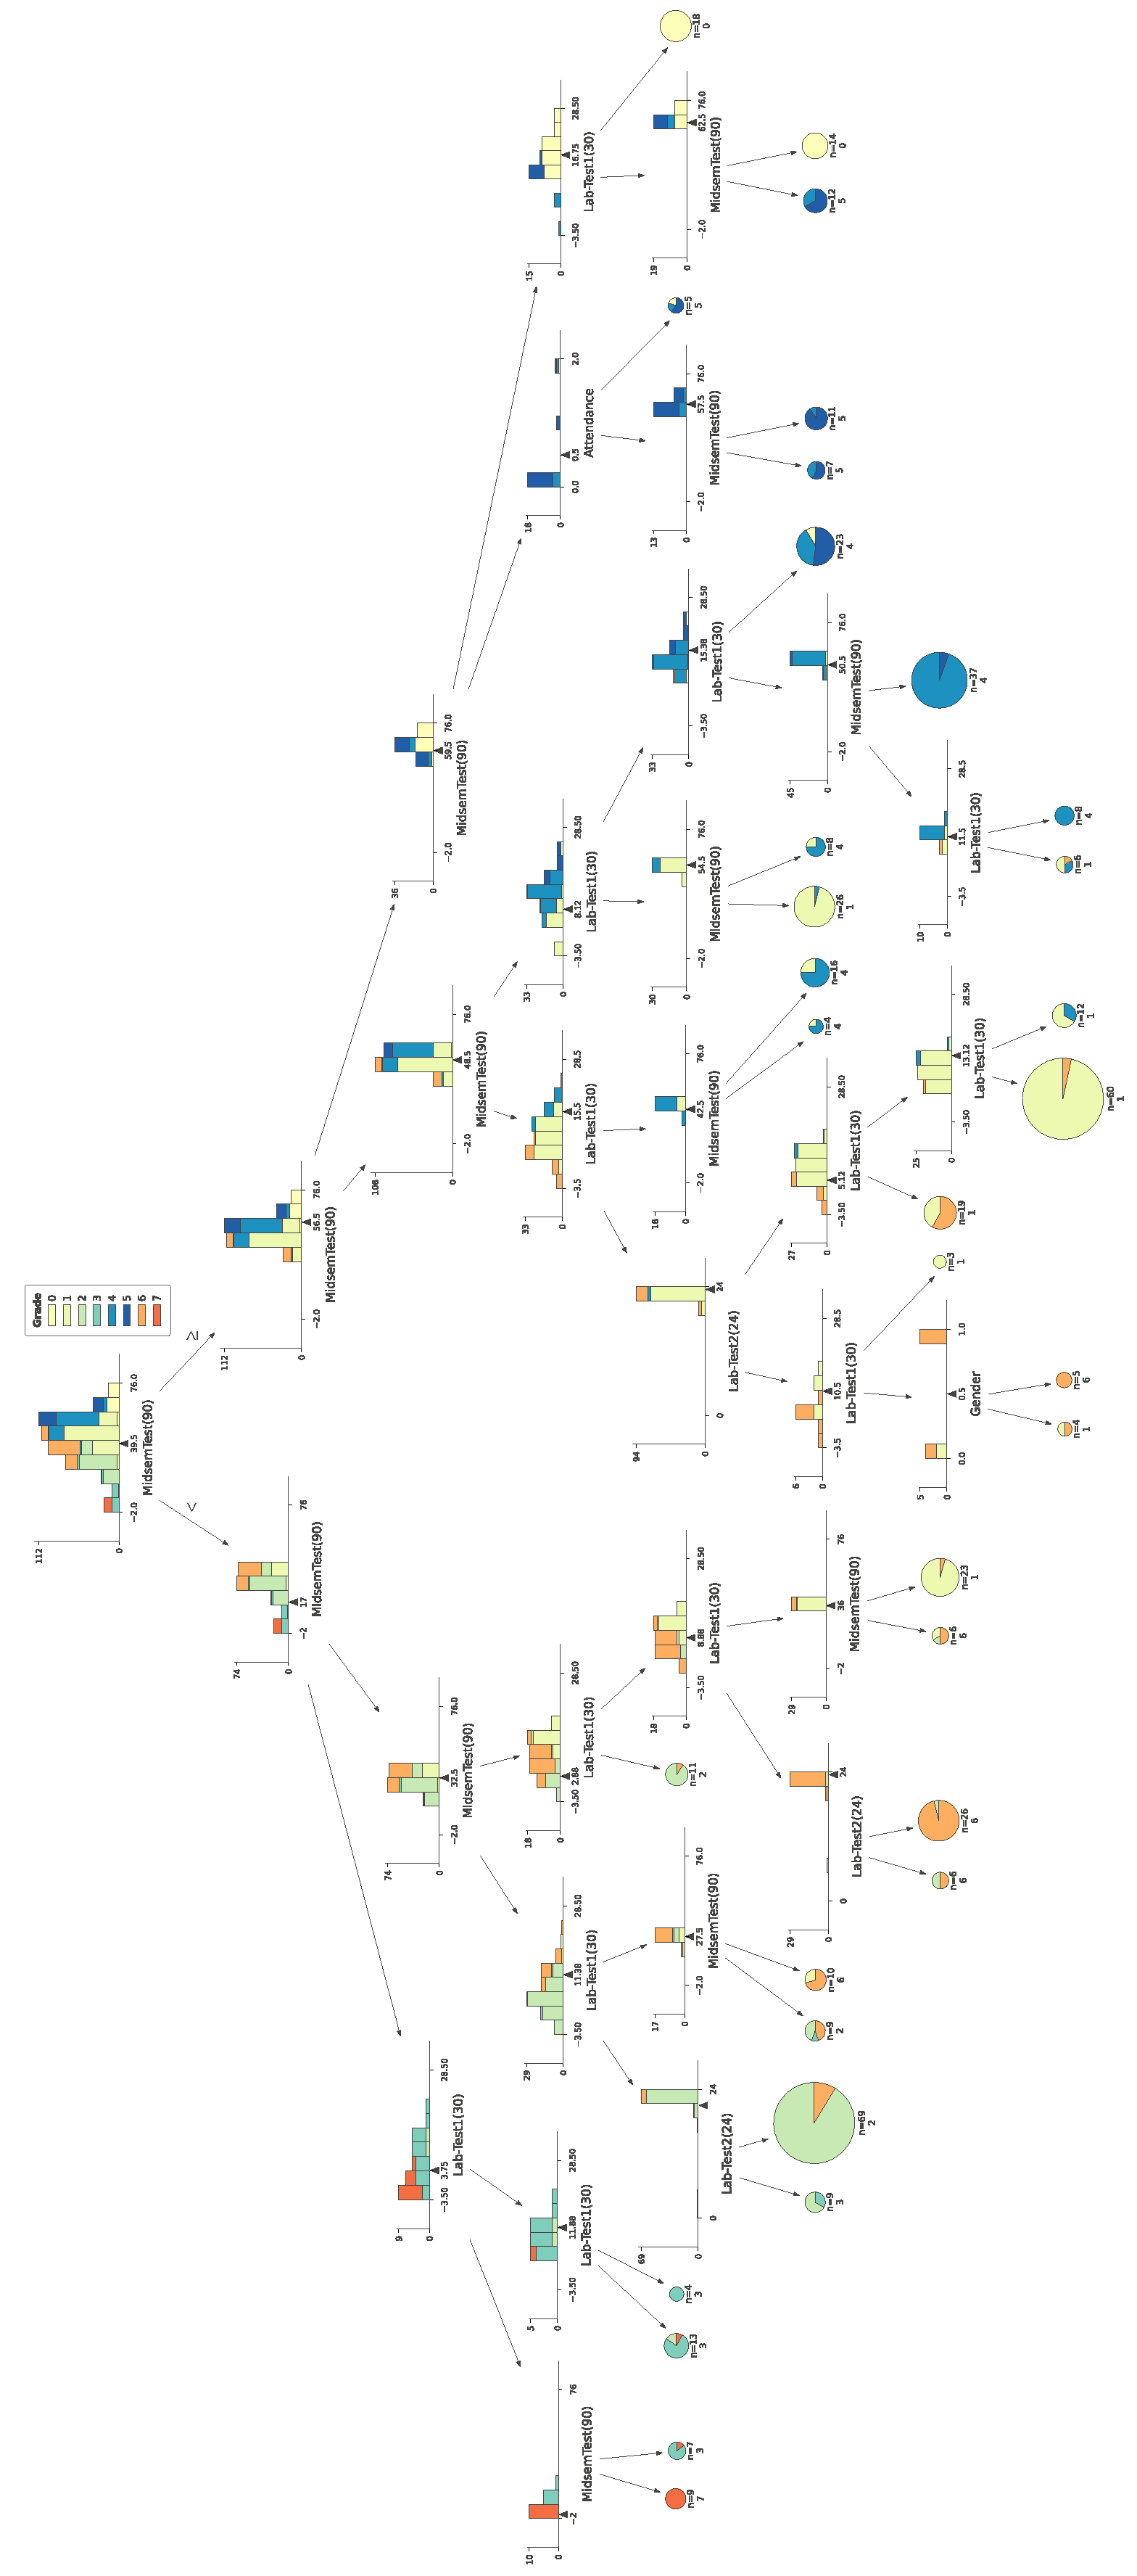
\includepdf[pages=-]{images/rf_viz_cmodel.pdf}